Error-resilience is typically a topic discussed orthogonally to congestion
control and the main reason is that, error-resilience caters to handling
packet loss while congestion control caters to the amount of information sent
over the network. This chapter is based on our work on unifying
error-resilience and congestion control.

In \citepub{c:err}, we evaluate the performance of the various
error-resilience schemes available for use in interactive multimedia
communication (mainly applicable to H.264). These are: using Negative
Acknowledgement (NACK) or Packet Loss Indication (PLI), Forward Error
Correction (FEC) or Unequal Level of Protection (ULP), adaptive slice sizes,
and Reference Pictures Selection Indication (RPSI). We evaluate the
performance of the proposed mechanisms in diverse scenarios in a simulated
environment (in ns-2) using real-world 3G loss patterns~\cite{3gppSim}.
Lastly, based on our observations, we define the applicability of the various
error-resilience with respect to end-to-end latency and packet loss.

In \citepub{c:fecrc}, we propose using FEC not only for error-resilience but
also for congestion control. Instead of probing for available capacity by
increasing the sending rate of the media flow, we propose introducing
redundancy. If a packet gets lost and the added FEC packet arrives in time the
receiving endpoint would recover the lost packet. However, if the packet is
not lost, by introducing the FEC packet the sender not only discovers that
there is additional available capacity, but also has a sense of the magnitude
(at minimum) of the available capacity. We compare our proposal with our
previous work in \citepub{c:3grc} and \citepub{c:hetrc}, and Google's
congestion control~\cite{draft.rrtcc}. We evaluate the performance of the
mechanisms in diverse scenarios implemented in a simulation environment (in
ns-2) and in our testbed.

\section{Error-resilience Schemes}
% explain all 4 and the adaptivity

H.264~\cite{h264} uses various error-control methods~\cite{err_res_h264_std,
wang98error, wang00review, 310669} to overcome loss due to bit-error
corruption (e.g., in wireless) and non-bursty packet loss (e.g., due to
congestion). These methods are classified into three categories: source
coding, channel coding, and joint source and channel methods. Source coding
refers to the methods implemented by the video codec. Channel coding refers to
the methods implemented by the networking layer. Joint source-channel refers
to methods that combine source-coding and network-coding mechanisms.

The H.264/AVC codec has several features that support error resilient
mechanisms for video communication that correspond to the above
categorization~\cite{310669}. At the codec level, the following are available:
adaptive slice size, Reference Picture Selection (RPS), and Flexible
Macroblock Ordering (FMO)~\cite{err_res_h264_std, wenger_ott_jscc}. Similarly,
at the channel level, the following are available: Selective Retransmission
(NACK), Packet Loss Indication (PLI). An example of joint source-channel is
Unequal Error Protection (UEP) with FEC~\cite{wang00review}, the sender
attempts to selectively protect important parts of the bitstream or by
encoding redundant pictures differently than other pictures \cite{ervcuupkp}.

The performance of the available error-resilience mechanisms vary with the
observed end-to-end latency, link loss, bandwidth constraints and operating
environment (3G/LTE to 3G/LTE, 3G/LTE to WLAN, or wireless to fixed, etc.). No
single error repair mechanism fits all operating environments. A solution that
works for an observed packet loss ratio of less than 2\%, may not scale well
for paths with higher packet loss or higher latency.

% The combination of end-to-end delay requirements, capacity constraints and
% varying packet loss rate require different error resilience mechanisms.

\begin{figure}
\centerline {
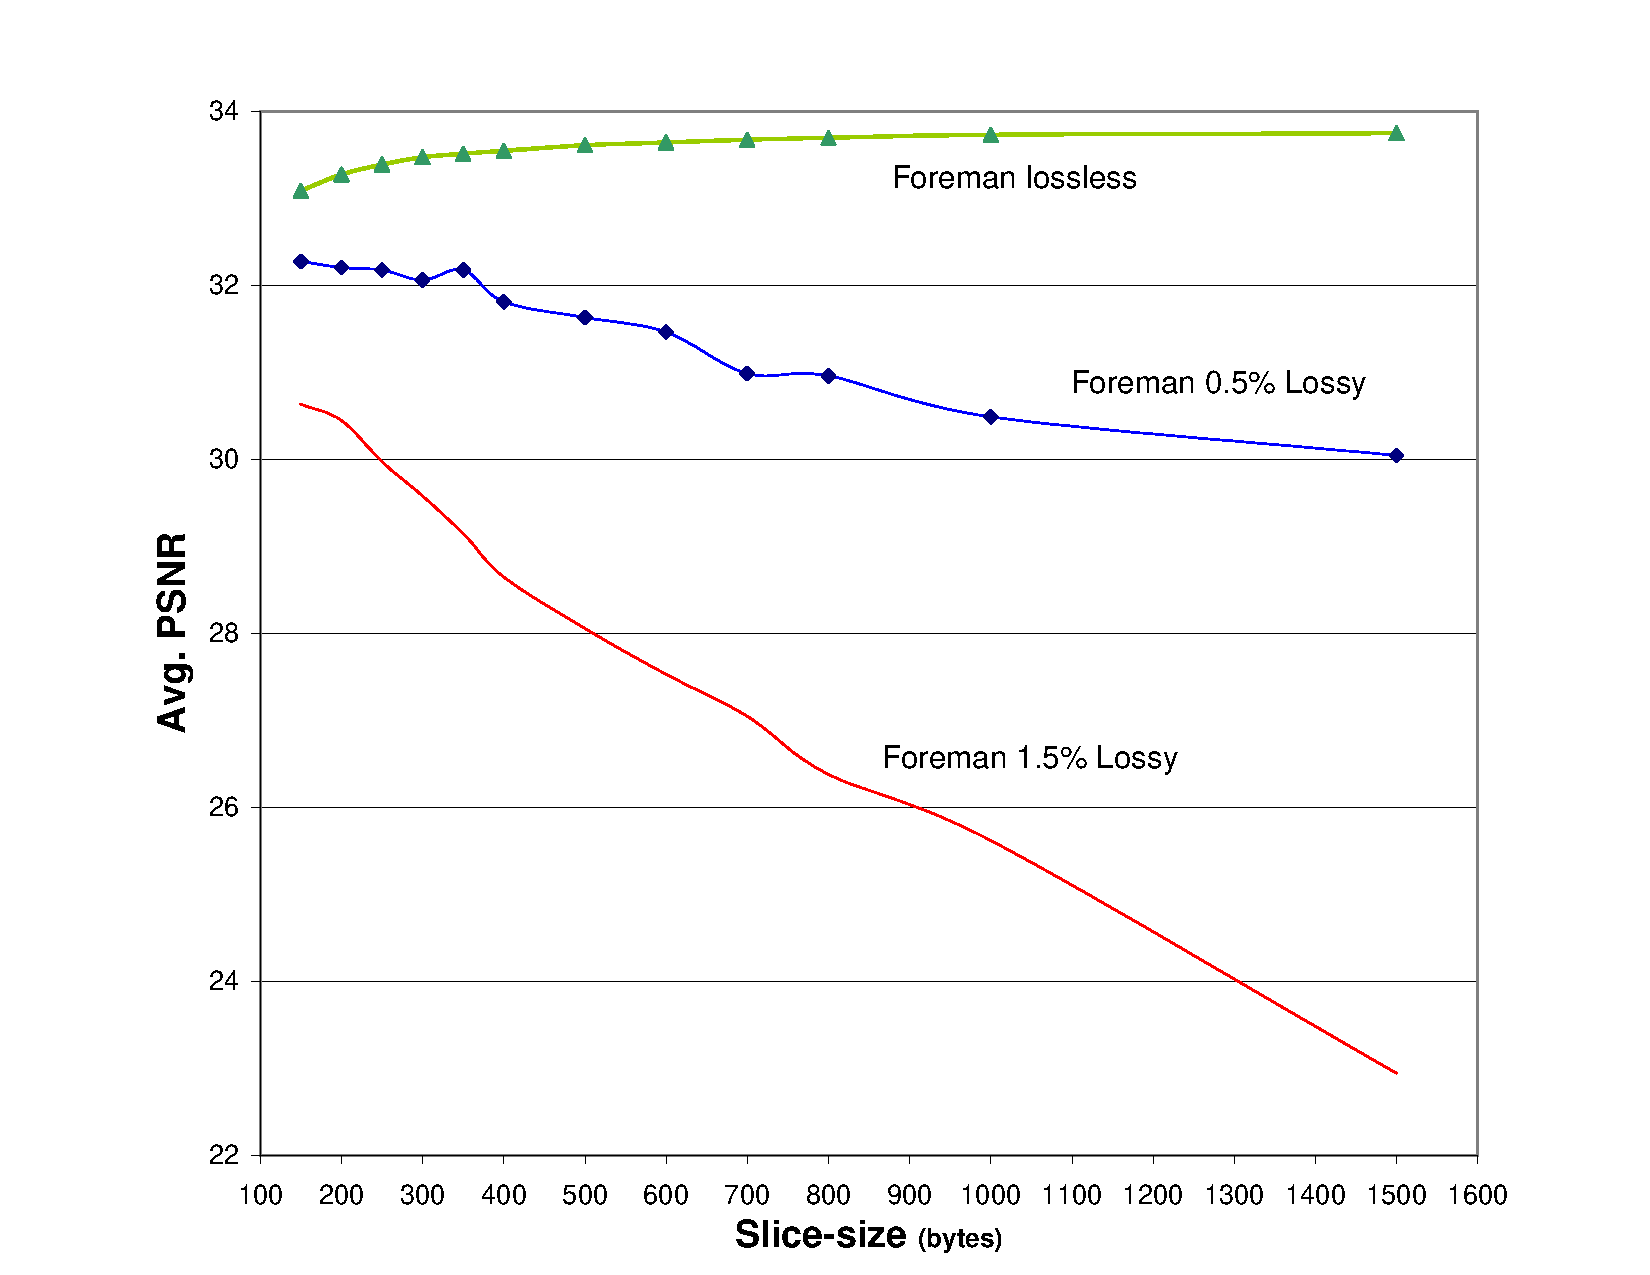
\includegraphics[width=0.66\textwidth]{chap6-graph-slicesize_mot}
}
\caption{Effect of different slice sizes on PSNR for links observing bit-error
corruption.}
\label{fig:slicesize_mot}
\end{figure}

\begin{itemize}
\setlength{\itemsep}{0pt}

  \item \textbf{\texttt{Retransmissions}}: In RTP, retransmissions are either
  payload-specific or at the transport-specific. Transport-specific loss
  contains packet loss information (Generic NACK), while payload-specific loss
  contains Slice Loss Information (SLI), Picture Loss Information (PLI) or
  Reference Picture Selection indication (RPS). Typically, the receiver
  detects a loss and sends it as soon as the RTCP reporting interval allows
  feedback.

  \item \textbf{\texttt{Adapting Slice Sizes}}: the encoder adapts the size of
  the picture slice based on the link characteristics; when the channel is
  lossless there can be one picture per slice or be the MTU size and when the
  high losses are reported, the slices are reduced in size (up to 100 bytes).
  Larger slice sizes improve encoding efficiency, but are more vulnerable to
  frame losses. Figure~\ref{fig:slicesize_mot} shows the variation of average
  PSNR with respect to different slice-sizes in varying loss scenarios. We
  observe, that there is direct correlation between packet loss and slice
  size.

  \item \textbf{\texttt{Reference Picture Selection}}: Instead of
  retransmitting the lost packet, the encoder finds the list of correctly
  received pictures by the decoder. Hence, for subsequent encodings, the
  encoder uses a different decoded picture for inter prediction reference.
  This method stops the temporal error propagation caused by an earlier packet
  loss. In the RPS message, the decoder either reports the list of pictures
  that were correctly received or lost. Hence, the encoder is able to retrieve
  the required picture loss data. The mode of operation can be decided
  depending on the observed packet loss rate.

  \item \textbf{\texttt{Unequal Error Protection}}: When the link latency is
  high, retransmissions cannot be used. In high latency networks, the
  retransmitted packets arrive too late to be played back. In these cases, the
  sender proactively uses a portion of the available capacity to send
  redundant packets (typically, FEC), hoping to recover any lost packet before
  decoding. Hence, by using UEP, the media senders try to strike a balance by
  protecting only a chosen set of the media packets. In \citepub{c:err}, we
  protect the reference frames and not the non-reference frames with UEP.

\end{itemize}

In \citepub{c:err}, we observe that 15-30\% of the lost packets are be
recovered for an end-to-end latency of 60ms (meeting the 150ms playout
deadline). The number of recovered packets be increased by reducing the RTCP
reporting interval, in this paper we use \emph{1s} reporting interval, with
early and immediate reporting as defined in \cite{rfc4585}. Based on these
experiments, it shows that NACK is an effective mechanism for low end-to-end
latency scenarios. Similarly, protecting the media flows with UEP incurred a
15-25\% overhead, and about 21-24\% of the lost packets were recovered.

\begin{figure}
\centerline {
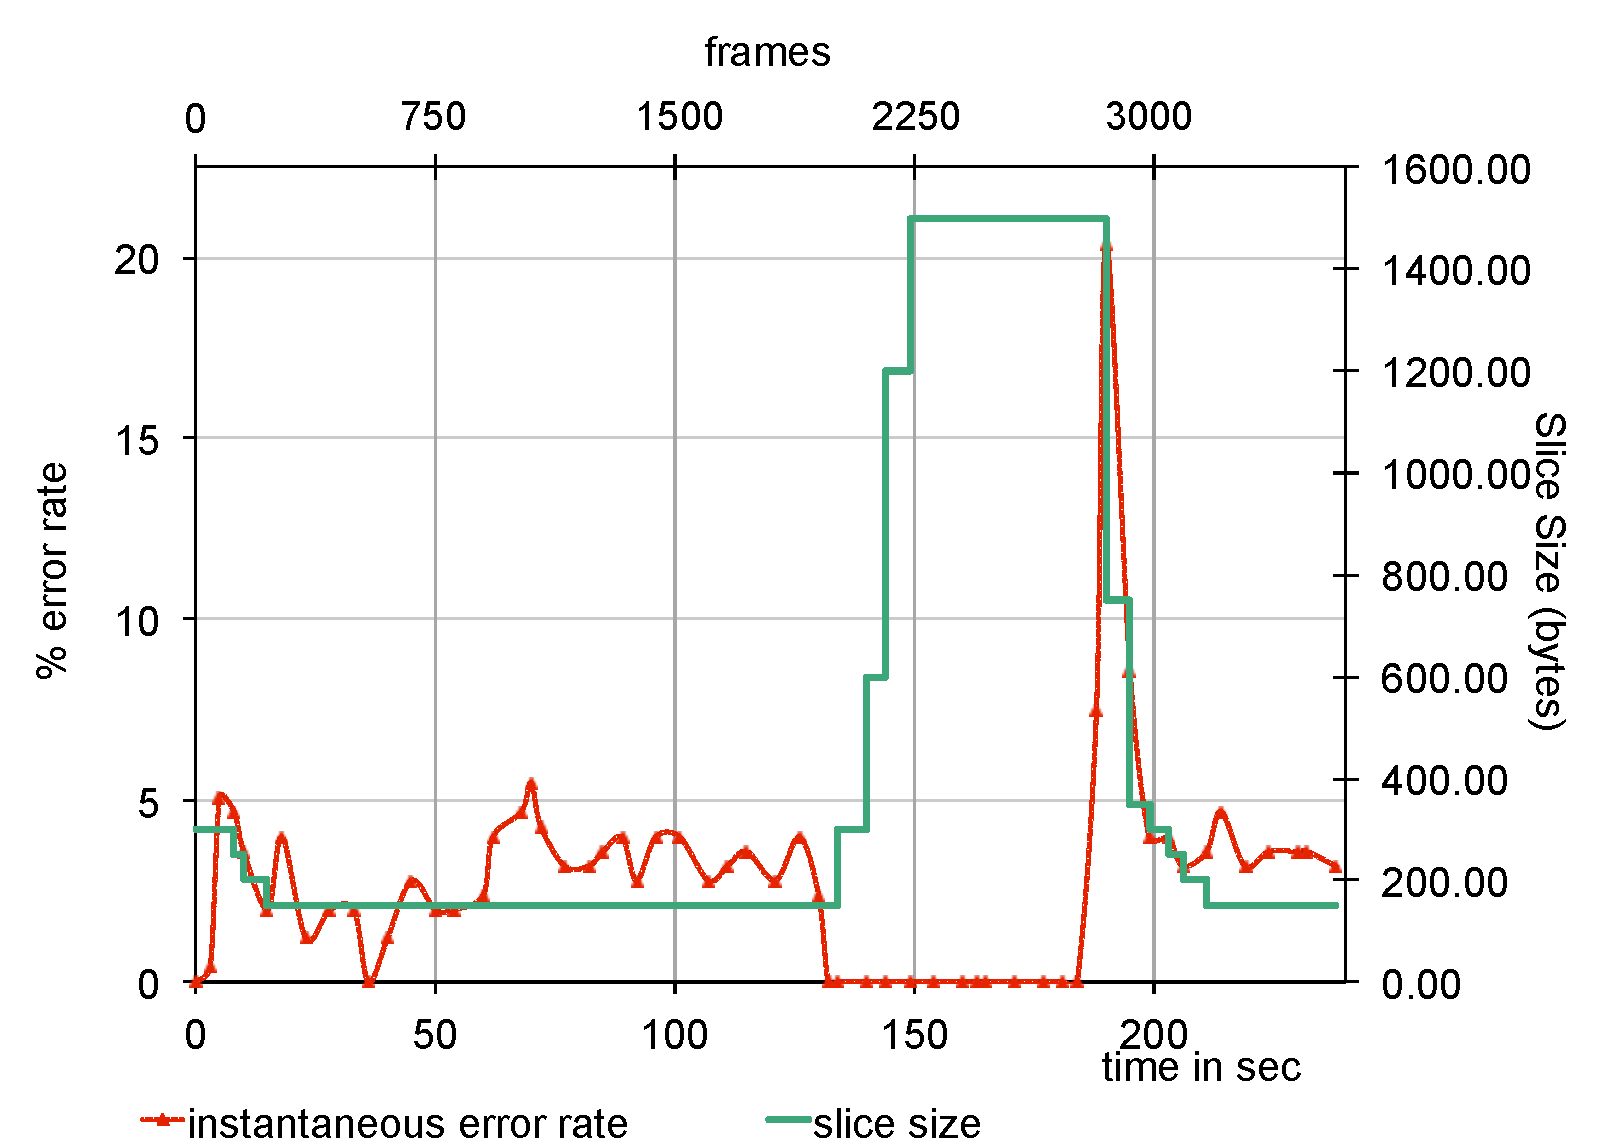
\includegraphics[width=0.66\textwidth, 
    clip=true, trim=0cm 0cm 0cm 2.5cm]{chap6-graph-ssa_adapt}
}
\caption{Adapting Slice Sizes due to variable error rates.}
\label{fig:ssa_adapt}
\end{figure}

Senders use a moving average of the last three observed fraction loss rate
reported in the RTCP RR to vary the slice size. The slice size is doubled for
every period with average loss below 1.0\% until it reaches the MTU size
(1500 bytes). Slice sizes remain constant for loss rates between 1\% to 2.5\%
to provide stability to the receiving system. However, In high loss scenarios,
if the slice size is larger than 400 bytes, it is halved and for sizes below
400 bytes, it is reduced in steps of 50 bytes to a minimum of 150 bytes. The
Figure ~\ref{fig:ssa_adapt} shows variation of slice-size with the
instantaneous loss rate and the average loss rate. Hence, by adapting the
slice sizes, the sender is not repairing the stream (or replacing the missing
packets), rather it is attempting to constrain the area of errors in the
picture. If an RTP packet containing a small sized slice is lost, a smaller
area of the decoded picture is affected, alternatively, when a packet
containing a large sized slice is lost, a large or complete decoded picture is
affected.

Lastly, using RPS error-resilience mechanism, the receiver indicates the
decoding correctness; when losses occur, which pictures or slices have been
decoded correctly or incorrectly. The feedback messages is encapsulated in an
RTCP packet and are reported to the sender. In our experiments, the receiver
reports RTCP every 250ms and it approximately consumes 2\% of the session
media rate. In Figure ~\ref{fig:rpsi_sim} (a), (b) and (c) we observe that the
PSNR drops down when a lost frame is referenced and the PSNR increases
immediately after the encoder chooses a correct reference picture. When the
one-way latency is 100 ms and the frame rate is set to 15 frames per second,
we observe the error propagation is stopped by RPS in about 4 to 7 pictures.


\begin{figure}[!t]
  \centerline{
  \subfloat [Foreman]{
    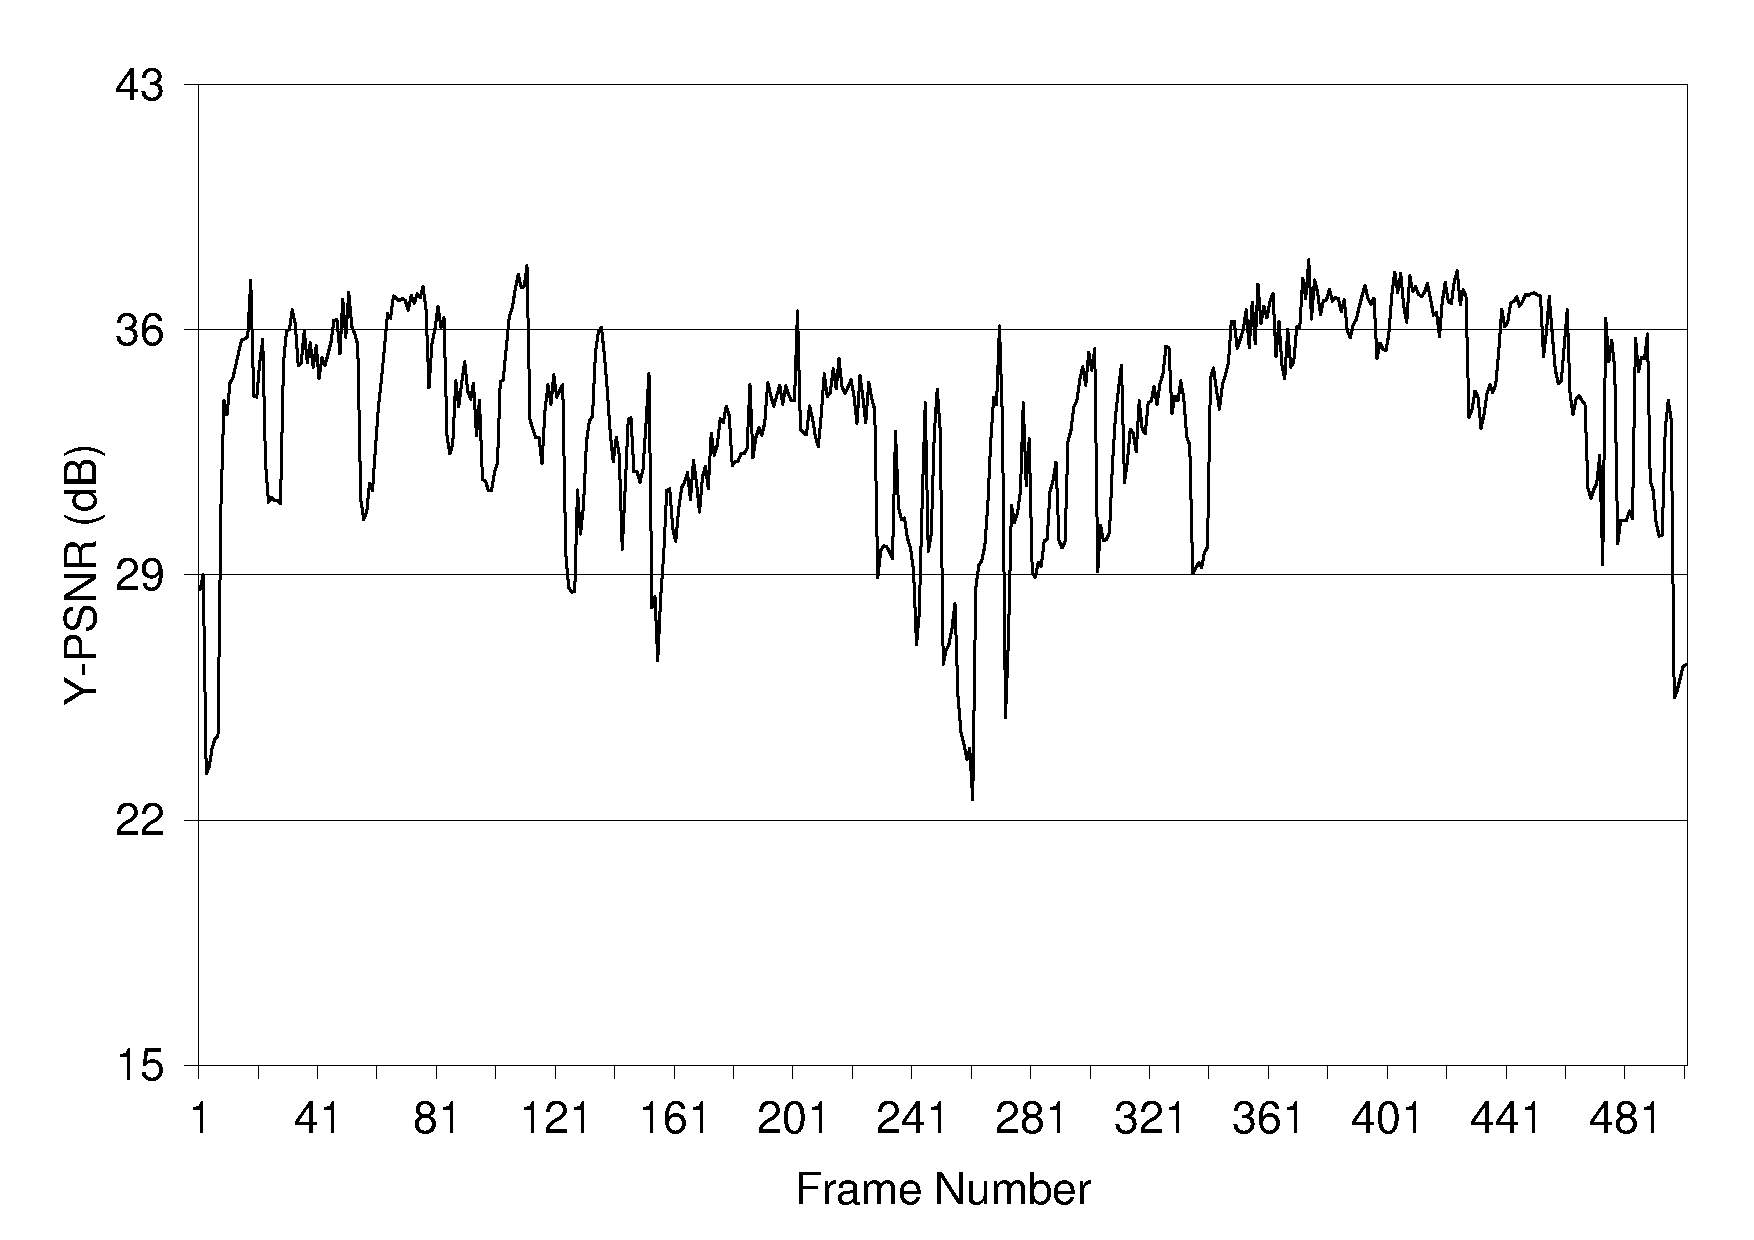
\includegraphics[width=0.33\textwidth]{chap6-graph-rpsi-1}
  } 
  \subfloat [News]{
    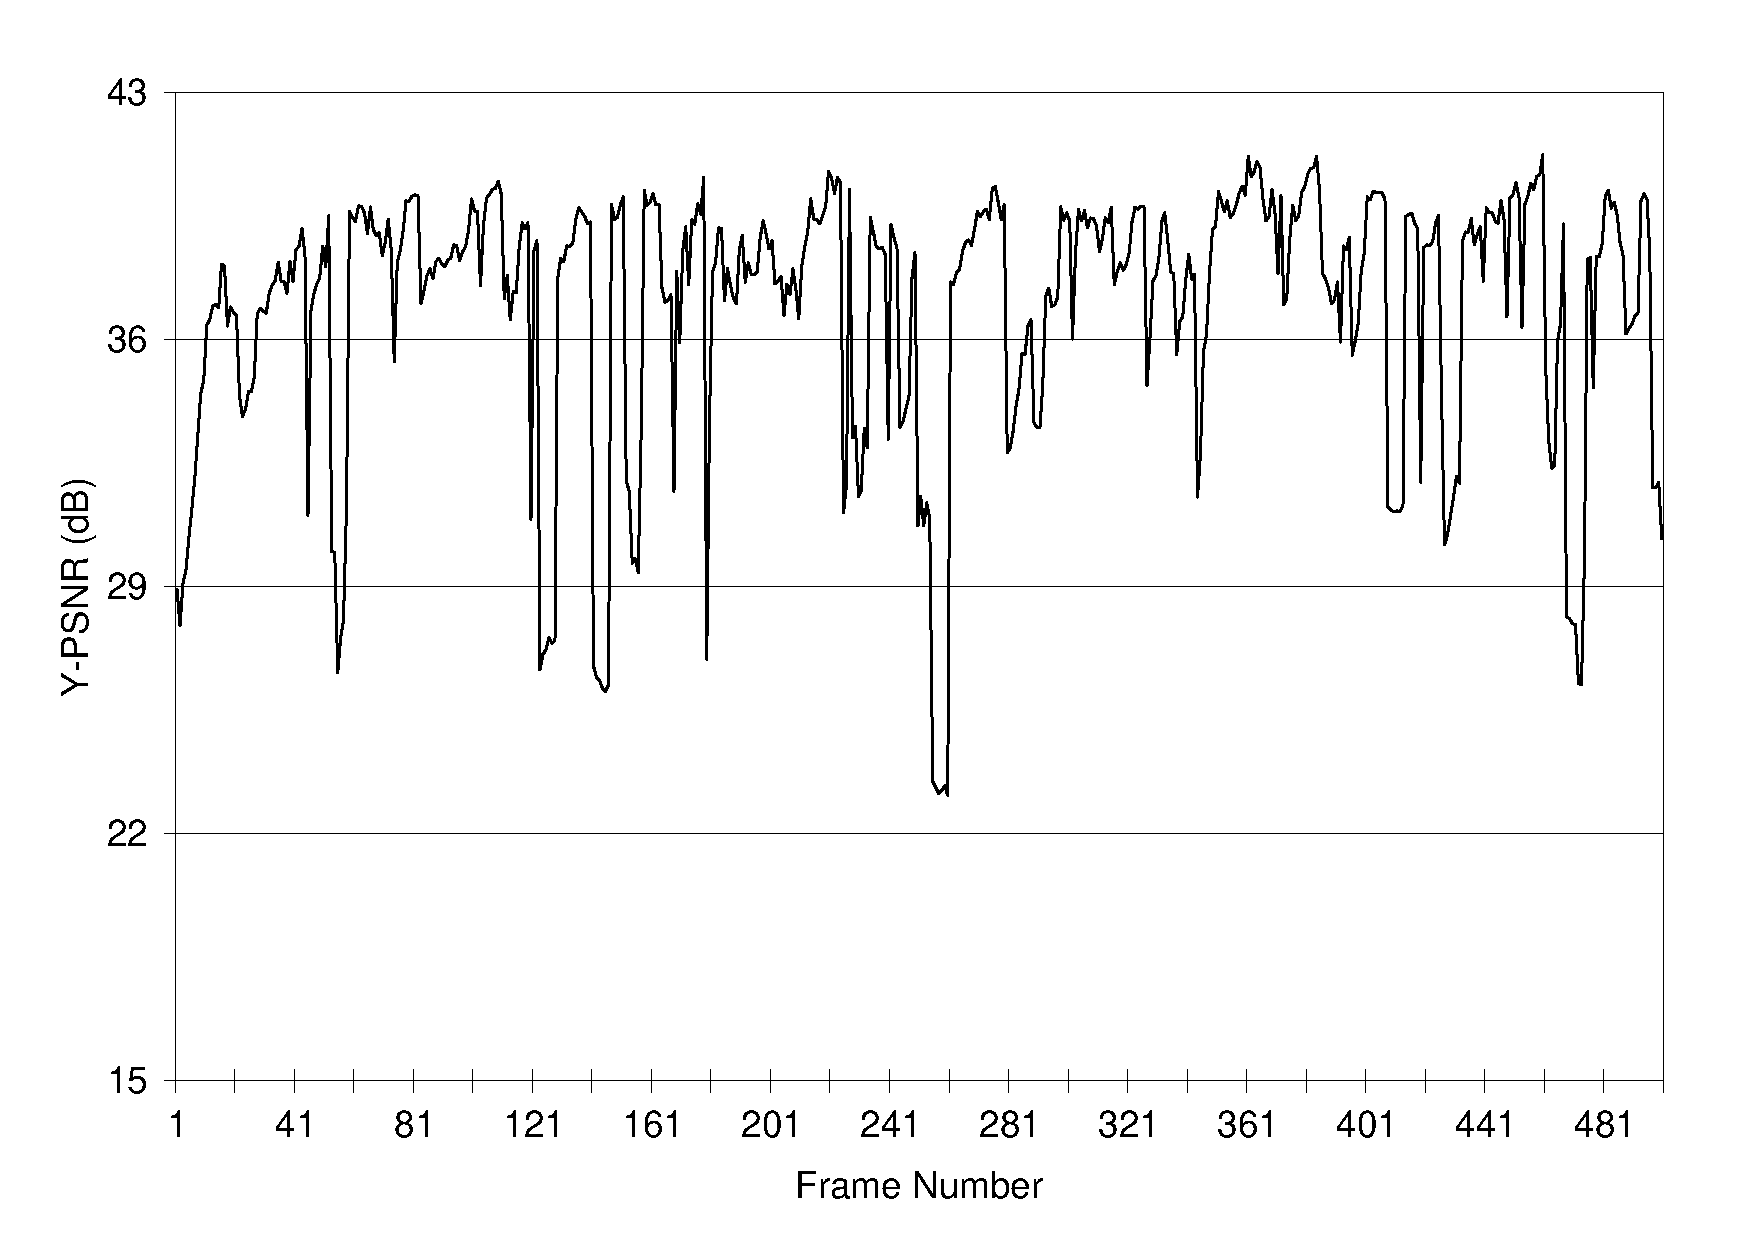
\includegraphics[width=0.33\textwidth]{chap6-graph-rpsi-3}
  }
  \subfloat [Football]{
    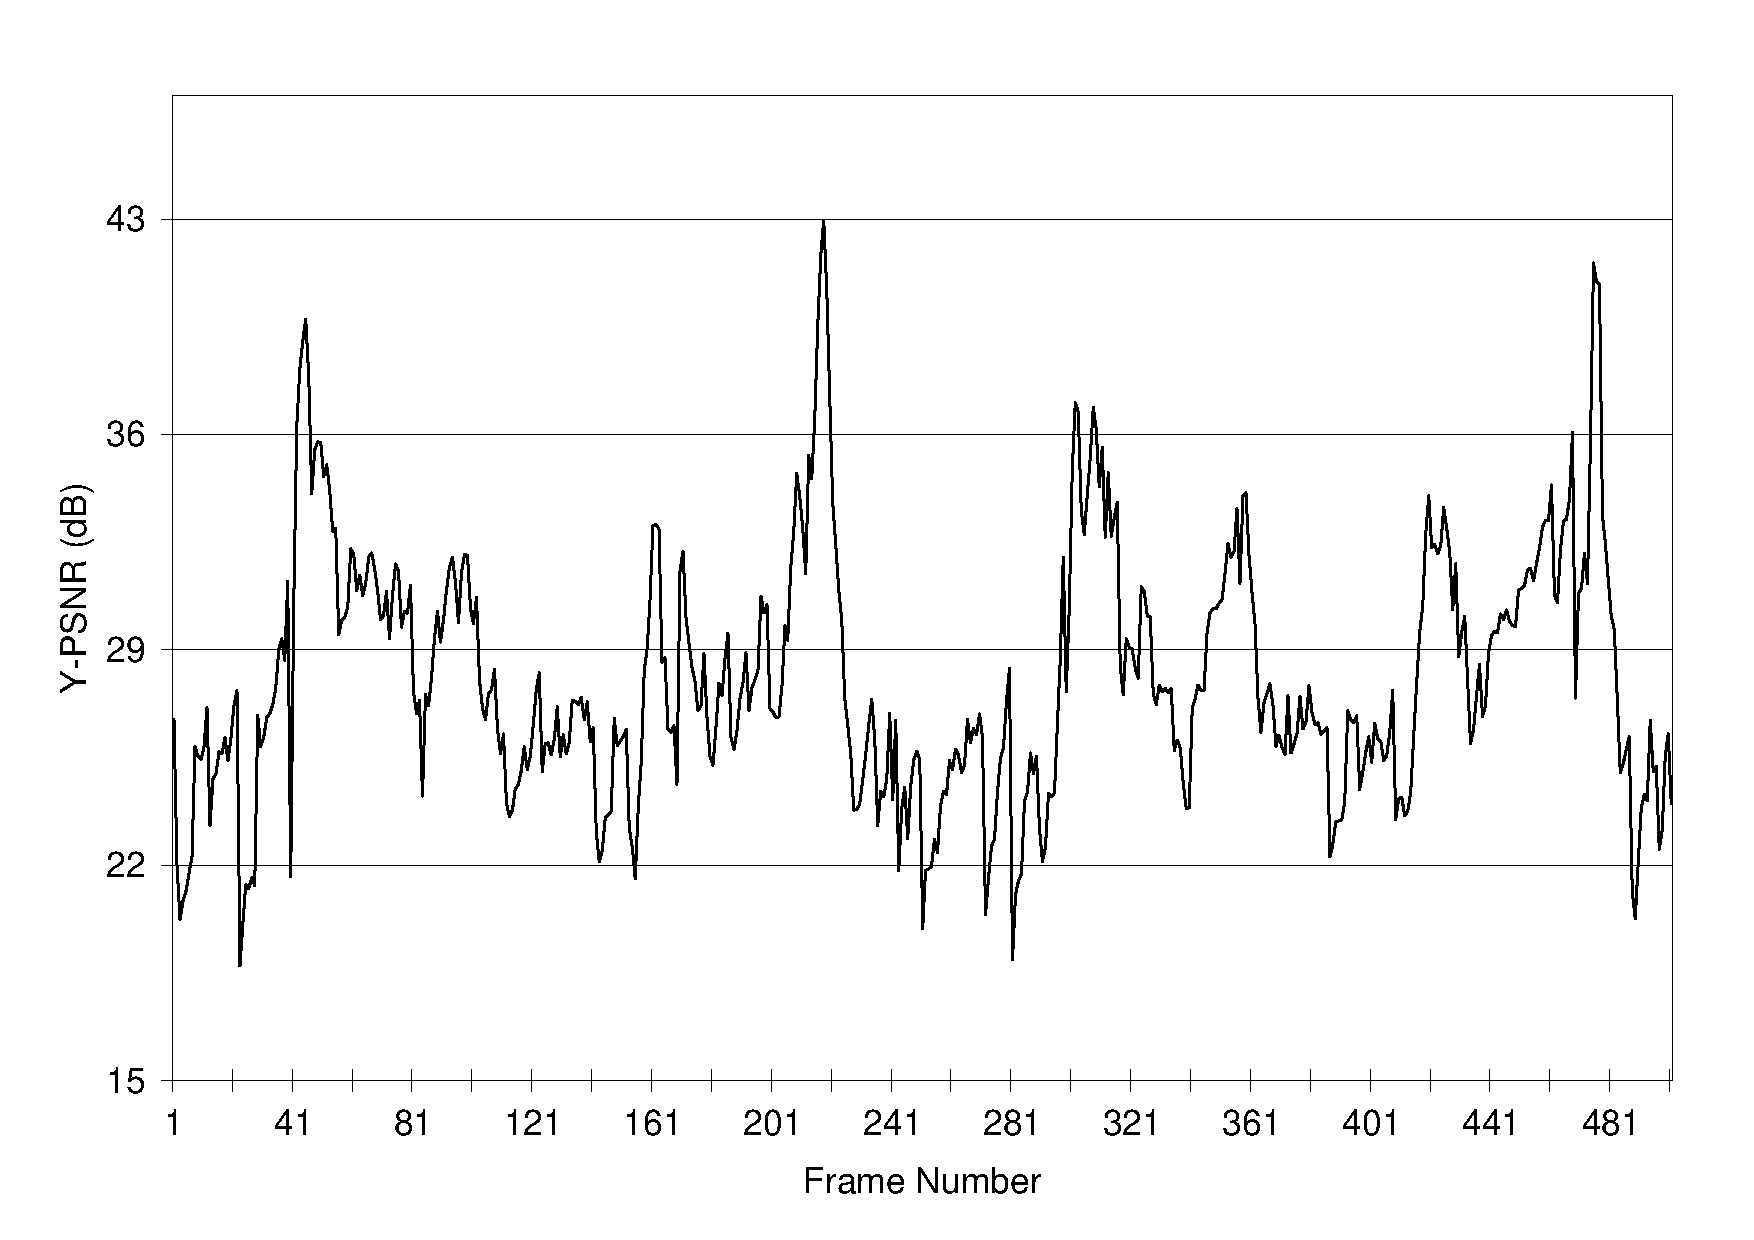
\includegraphics[width=0.33\textwidth]{chap6-graph-rpsi-5}
  }
}
\caption{PSNR Variation due to RPSI for (a) Foreman, (b) News, and (c)
Football sequences.}
\label{fig:rpsi_sim}
\end{figure}

Table~\ref{tab:err-sch-psnr} presents the average PSNR of the different error
resilience schemes for links with 0.5\% fractional loss. We observe that the
RPS performs better than UEP and NACK and is comparable to adaptive slices.
The UEP underperforms mainly because the media stream is encoded at a lower
rate to make room for FEC, compared to the media streams of the other
error-resilience mechanisms.

\begin{table}
  \centering{
  \scalebox{0.9}{
\begin{tabular}{cccc}
\hline
 & \multicolumn{3}{l}{Y-PSNR, 0.5\% PLR} \\
\hline
 & Foreman & Football & News  \\
NACK & 32.1456 & 28.0331 & 35.3867 \\
RPSI & 33.68 & 28.05 & 37.37 \\
UEP & 28.33 & 26.86 & 34.47 \\
Adaptive slices & 32.30 & 28.4 & 37.25 \\
\hline
\end{tabular}
}}
\caption{Comparing the performance of different error-resilience
schemes on three different types of YUV sequences~\cite{YUV_seq}. The link
loss rate is 0.5\% at each 3G link.}
\label{tab:err-sch-psnr}
\end{table}

In \citepub{c:err}, we model the error-resilience mechanisms as a function of
observed packet loss and end-to-end delay (or latency) and
Figure~\ref{fig:apply_err} summarizes the applicability of the
error-resilience mechanisms based on our experiments. NACK is useful when loss
rates are low and the end-to-end delay is also low. Adaptive slice size (SSA)
is applicable to the whole operational region because it attempts to scale the
packet size based on the observed loss rate, but does not help in packet
repair. RPS works better on links with bursty packet loss, where NACK would
not be effective. By correctly choosing a new reference picture, the sender is
more effective when network latency is higher. UEP/FEC is mainly useful when
the sender and receiver cannot effectively co-operate to repair the stream and
the fractional loss is within the FEC's chosen protection range.

\begin{figure}
\centerline {
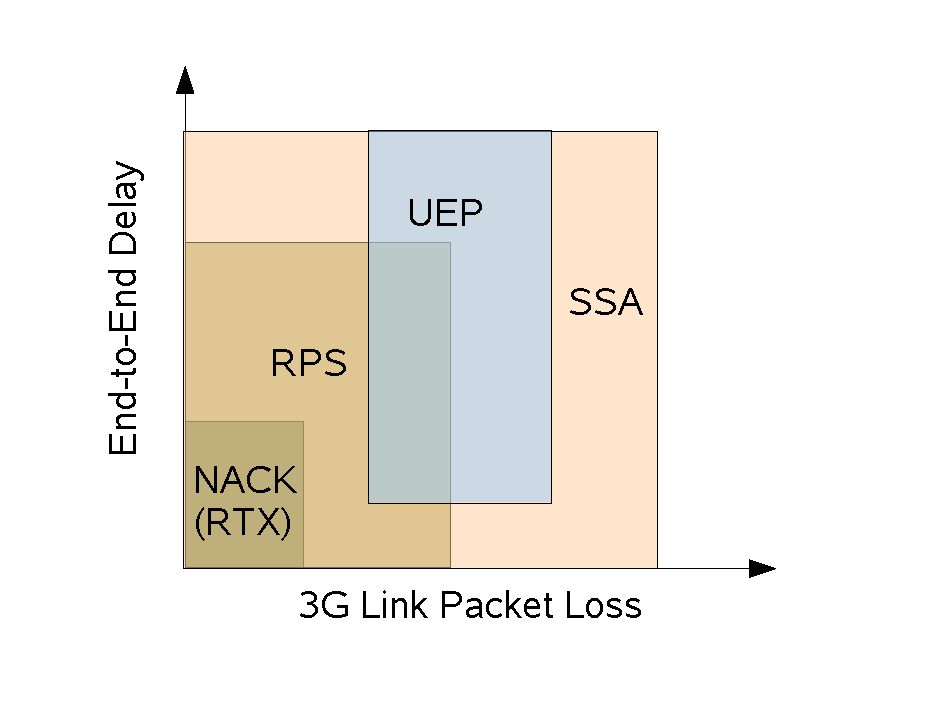
\includegraphics[width=0.75\textwidth, 
    clip=true, trim=0cm 1cm 0cm 1cm]{chap6-fig-apply-err}
}
\caption{Applicability of the error-resilience schemes in heterogeneous
environment containing both wireless and wired links.}
\label{fig:apply_err}
\end{figure}


\section{Using FEC for Congestion Control}

% Figure with the idea: FEC for CC

% Table of FEC, C-NADU and RRTCC :)